\documentclass[a6paper]{minimal}
\usepackage{chemfig}
\usepackage[version=4]{mhchem}
\usepackage{tikz}
\usepackage{fontspec}
\usepackage[landscape]{geometry}
\setmainfont{Hiragino Sans GB}
\usetikzlibrary{positioning}

\begin{document}
	\begin{center}
	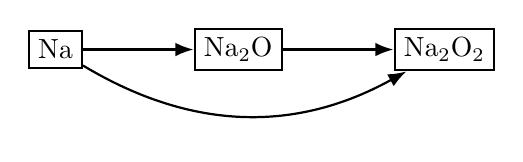
\begin{tikzpicture}[node distance=40pt, auto, thick]
		\node[draw] (Na) {\ce{Na}};
		\node[draw, right=of Na] (Na2O) {\ce{Na2O}};
		\node[draw, right=of Na2O] (Na2O2) {\ce{Na2O2}};

		\draw[-Latex] (Na) to (Na2O);
		\draw[-Latex] (Na2O) to (Na2O2);
		\draw[-Latex] (Na) to[bend right] (Na2O2);
	\end{tikzpicture}
	\newline
	
	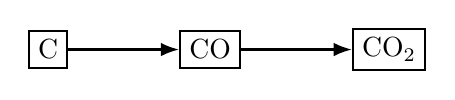
\begin{tikzpicture}[node distance=40pt, auto, thick]
		\node[draw] (C) {\ce{C}};
		\node[draw, right=of C] (CO) {\ce{CO}};
		\node[draw, right=of CO] (CO2) {\ce{CO2}};

		\draw[-Latex] (C) to (CO);
		\draw[-Latex] (CO) to (CO2);
	\end{tikzpicture}
	\newline
	
	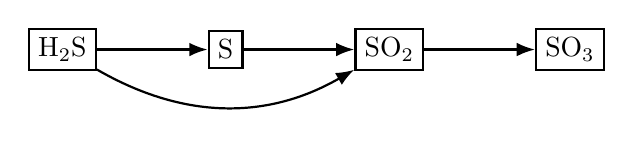
\begin{tikzpicture}[node distance=40pt, auto, thick]
		\node[draw] (H2S) {\ce{H2S}};
		\node[draw, right=of H2S] (S) {\ce{S}};
		\node[draw, right=of S] (SO2) {\ce{SO2}};
		\node[draw, right=of SO2] (SO3) {\ce{SO3}};

		\draw[-Latex] (H2S) to (S);
		\draw[-Latex] (S) to (SO2);
		\draw[-Latex] (SO2) to (SO3);
		\draw[-Latex] (H2S) to[bend right] (SO2);
	\end{tikzpicture}
	\newline
	
	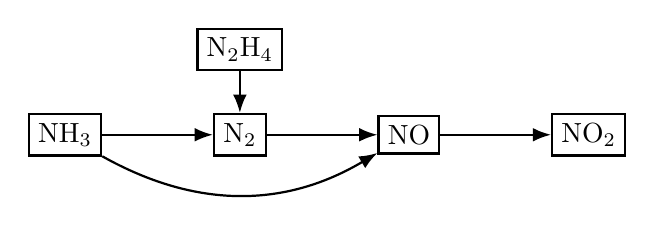
\begin{tikzpicture}[node distance=40pt, auto, thick]
		\node[draw] (N2H4) {\ce{N2H4}};
		\node[draw, below=15pt of N2H4] (N2) {\ce{N2}};
		\node[draw, left=of N2] (NH3) {\ce{NH3}};
		\node[draw, right=of N2] (NO) {\ce{NO}};
		\node[draw, right=of NO] (NO2) {\ce{NO2}};

		\draw[-Latex] (N2H4) to (N2);
		\draw[-Latex] (NH3) to (N2);
		\draw[-Latex] (N2) to (NO);
		\draw[-Latex] (NO) to (NO2);
		\draw[-Latex] (NH3) to[bend right] (NO);
	\end{tikzpicture}
	
	\end{center}
\end{document}